\documentclass[times, utf8, zavrsni]{fer}
\usepackage{booktabs}
\usepackage{listings}
\usepackage{xcolor}
\usepackage{graphicx}
\graphicspath{ {./notes/screenshots/} }

\colorlet{punct}{red!60!black}
\definecolor{background}{HTML}{EEEEEE}
\definecolor{delim}{RGB}{20,105,176}
\colorlet{numb}{black!60!black}

\lstdefinelanguage{json}{
    basicstyle=\normalfont\ttfamily,
    numbers=left,
    numberstyle=\scriptsize,
    stepnumber=1,
    numbersep=8pt,
    showstringspaces=false,
    breaklines=true,
    frame=lines,
    backgroundcolor=\color{background},
    literate=
     *{0}{{{\color{numb}0}}}{1}
      {1}{{{\color{numb}1}}}{1}
      {2}{{{\color{numb}2}}}{1}
      {3}{{{\color{numb}3}}}{1}
      {4}{{{\color{numb}4}}}{1}
      {5}{{{\color{numb}5}}}{1}
      {6}{{{\color{numb}6}}}{1}
      {7}{{{\color{numb}7}}}{1}
      {8}{{{\color{numb}8}}}{1}
      {9}{{{\color{numb}9}}}{1}
      {:}{{{\color{punct}{:}}}}{1}
      {,}{{{\color{punct}{,}}}}{1}
      {\{}{{{\color{delim}{\{}}}}{1}
      {\}}{{{\color{delim}{\}}}}}{1}
      {[}{{{\color{delim}{[}}}}{1}
      {]}{{{\color{delim}{]}}}}{1},
}
\lstset{
  language=bash,
  basicstyle=\ttfamily,
  breaklines=true,
  showstringspaces=false,
  numbers=left,
  stepnumber=1,
  numbersep=8pt,
  frame=lines,
  backgroundcolor=\color{background},
  numberstyle=\scriptsize
}

\begin{document}

% TODO: Navedite broj rada.
\thesisnumber{000}

% TODO: Navedite naslov rada.
\title{Usporedba performanci Ethereum raspodijeljene knjige na raznorodnom sklopovlju}

% TODO: Navedite vaše ime i prezime.
\author{Jakov Buratović}

\maketitle

% Ispis stranice s napomenom o umetanju izvornika rada. Uklonite naredbu \izvornik ako želite izbaciti tu stranicu.
\izvornik

% Dodavanje zahvale ili prazne stranice. Ako ne želite dodati zahvalu, naredbu ostavite radi prazne stranice.
\zahvala{Zahvaljujem se mentoru doc. dr. sc. Igoru Čavraku na podršci i pomoći pri izradi ovog rada.\\
Zahvaljujem se i kolegi Ediju Sinovčiću koji se već dulje vrijeme bavi razvojem programskih rješenja
koji koriste tehnologiju distribuirane knjige te mi je mogao odgovoriti i riješiti sve moje nedoumice.\\
}

\tableofcontents

\chapter{Uvod}
Ethereum mnogi znaju kao jednu od najpopularnijih kriptovaluta. Iako je to točno, Ethereum je mnogo
više od same digitalne valute. To je programska potpora raspodijeljena na mreži računala na kojima je
moguće razmjenjivati podatke i pokretati računalne programe bez centralnog poslužitelja. 
Podaci se repliciraju na svaki čvor u mreži. Određenim algoritmima konsenzusa se osigurava 
nepromjenjivost i pouzdanost. 
To omogućuje da mreža bude potpuno javna i sigurna. Posebnost je što svatko može koristiti
mrežu i objavljivati sadržaj bez ikakvih posebnih dozvola. \\ Za razliku od Bitcoina
i mnogih drugih implementacija tehnologije distribuirane knjige koji nude mogućnost pohrane podataka
bez centralnog poslužitelja, Ethereum mreža omogućuje i izvođenje programskog koda u obliku pametnih ugovora.\\
U ovom radu je prikazano kako se može pokrenuti privatna mreža na različitom sklopovlju s naglaskom
na ispitivanje najnižih zahtjeva sklopovlja. Dodatno, prikazat ću proces obavljanja transakcija
i izvođenja programskog koda na čvorovima uz prigodni prikaz sa sučeljem u jednostavnoj web aplikaciji.\\
U prvom poglavlju ovog rada, objasnit će se osnove tehnologije distribuirane knjige i njene primjene.\\
Nakon toga će biti poglavlje usmjereno na Ethereum kao implementaciju navedene tehnologije te prikaz
i opis njegovih algoritama konsenzusa. \\
Treće poglavlje je zaduženo za detaljan postupak kreiranja privatne mreže na raznorodnom sklopovlju
s različitim operativnim sustavima. \\
U posljednjem poglavlju je na prethodno kreiranu mrežu dodan grafički prikaz aktivnosti mreže i transakcija
u jednostavnoj web aplikaciji. 

\chapter{Tehnologija glavne raspodijeljene knjige}
U nastavku ćemo tehnologiju glavne raspodijeljenje knjige (engl. \emph{Distributed Ledger Technology})
 referencirati kraće po kratici engleskog naziva, odnosno DLT. \\ 
DLT i blockchain se češto poistovjećuju no to nije u potpunosti ispravno. Bitno je znati da je 
svaki blockchain DLT s određenim pravilima konsenzusa.
DLT je baza podataka repliciranog sadržaja na svakom čvoru \emph{peer-to-peer} mreže. Svaki čvor
mora sadržavati identičnu kopiju kompletnog sadržaja baze podataka i konstantno se ažurira sa susjednim
čvorovima. \\
Kod blockchaina se te promjene zapisuju u obliku transakcije u blokove koji formiraju neprekidan lanac.
Odatle dolazi i sam naziv tehnologije. Prije nego što se novi blok transakcija poveže u postojeći lanac
blokova, on mora biti potvrđen od većine čvorova prema poznatim pravilima konsenzusa koji se koristi
u toj implementaciji mreže. Nakon što je blok povezan, sve transakcije zabilježene ostaju zauvijek i
šanse za maliciozne izmjene su vrlo malene. Više o mogućim napadima će biti opisano u nastavku jer
se razlikuju za ovisno o implementaciji. \\
Bitcoin je najpoznatiji primjer primjene blockchaina u široj populaciji. Njegova mreža je aktivna 
od siječnja 2009. godine kada je Satoshi Nakamoto potvrdio prvi blok (engl. \emph{genesis}).
Još uvijek nije poznato tko je Satoshi Nakamoto i je li to uopće stvarna osoba ili naziv za grupu
ljudi koji su sudjelovali u tazvoju bitcoina. Problem koji bitcoin pokušava riješiti je centraliziranost
ekonomskog sustava i plaćanja. Svaka transkacija u trenutnom sustavu mora proći kroz centralno sjedište,
odnosno banku. To znači da korisnici moraju vjerovati centralnom sjedištu da će provesti transakcije
kako korisnik želi i da se neće ponašati maliciozno. Također, korisnici moraju vjerovati u sigurnost
centralnog sjedišta i mogućnost zaštite od napada od treće strane. \\
Za takav način je potreban velik broj ljudi, novca i kontrole što dovodi dodatna ograničenja kao što 
su čekanje na potvrdu transakcije dulje vrijeme, nemogućnost obavljanja transakcija vikendom i praćenje
toka novca. \\
Bitcoin te probleme rješava na način da izbacuje centralno sjedište i umjesto njega koristi \emph{Proof of Work}
pravila konsenzusa koja osiguravaju pouzdanost bez povjerenja. \\
Nakon bitcoina su se pojavili mnogi \emph{forkovi} s manjim ili većim promjenama, obično u veličini
samih blokova ili brzini potrvrđivanja istih. Oni su obilježili prvu generaciju kriptovaluta. \\
2013. godine ruski programer Vitalik Buterin predlaže Ethereum, novu javnu platformu koja koristi 
dorađeno izdanje Nakamotovog \emph{PoW} konsenzusnog algoritma. Posebnost Ethereuma jest da on nije
samo raspodijeljena platforma za transakcije, već raspodijeljeni virtualni stroj (engl. \emph{Ethereum Virtual Machine -EVM})
 koji može izvoditi kod poznat pod nazivom pametni ugovor (engl. \emph{smart contract}). \\



\chapter{Proof of Authority algoritam}

\chapter{PoA mreža na raznovrsnom sklopovlju}
Glavni zadatak ovog završnog rada bio je postaviti vlastitu mrežu koristeći Ethereum platformu na raznorodnom sklopovlju
te provjeriti koliko su visoki zahtjevi jedne takve mreže na hardver. Osim same mreže, dodane su još neke osnovne funkcionalnosti
kako bi se što ovi laboratorijski uvjeti što više približili pravom svijetu te nam ponudili kvalitetnije rezultate. Tako recimo
imamo postavljen pretražitelj blokova (engl. \emph{Block explorer}) koji u realnom vremenu prikazuje putem web aplikacije
trenutni blok i transakcije koje su se provele u tom bloku. Moguće je i pretraživati starije blokove putem njega. \\
Osim pretražitelja blokova, dodana je i još jedna web aplikacija koja nudi podatke o opterećenosti pojedinog čvora u mreži
što je korisno za ovaj završni rad jer jednostavno možemo usporediti opterećenost na raznorodnom sklopovlju. \\
Posljednja funkcionalnost jest zapravo podizanje (engl. \emph{deployment}) najjednostavnijeg pametnog ugovora kako bismo
zapravo mogli vidjeti samu komunikaciju između čvorova i izvođenje programskog koda.

\section{Sklopovlje i programska podrška}
Ono što čini ovaj sustav zanimljivim i pristupačnim širokoj populaciji je mogućnost sudjelovanja u distribuiranoj mreži s vrlo
različitim sklopovljem. To znači da korisnici u većini slučajeva neće morati ulagati novac u novi hardver.\\ U ovom radu su korištena
tri uređaja s ARM procesorima, jedno prijenosno računalo s Intel 64 bitnim procesorom i stolno računalo s AMD 64 bitnim procesorom.
\subsection{Cubieboard2}
Cubieboard2 jest jednostavno računalo (engl. \emph{single-board computer}) kompanije Cubietech. Ovo računalo jest otvoreno
što znači da su svi podaci o sklopovlju dostupni javno. Cubieboard2 je njihov drugi proizvod, izravni nasljednik originalnog Cubieboarda.\\
Pogoni ga Allwinner A20 čipset kojeg čini dvojezgreni Cortex-A7 procesor takta 1 GHz s Mali400 grafičkim sklopom. 
Na ploči je integrirana radna memorija DDR3 kapaciteta 1 GB na taktu 480 MHz i memorija za pohranu od 4 GB. Memorija za pohranu je 
proširiva microSD memorijskom karticom.
Ne postoji ugrađen modul za bežičnu povezivost putem Wifi-a pa je korišten Ethernet ulaz propusnosti 10M/100M. \\
Ovo računalo je moguće napajati putem USB micro sučelja ili DC 5V ulaza. \\
Obzirom da je Cortex-A7 ARM procesor postoje razne mogućnosti kad je u pitanju odabir operativni sustav. Tvornički dolazi
Android da unutarnjoj memoriji od 4 GB što nije odgovaralo potrebama ovog rada pa je bilo potrebno pronaći odgovarajuću distribuciju
Linux operativnog sustava.\\ Odličan izbor se pokazala distribucija armbian koja je ponudila minimalnu instalaciju operativnog sustava
za ovo računalo baziranu na Debian Linuxu. Dolazi s ažurnom verzijom Linux kernela 5.4 što znači da sa strane programske podrške
postoje dobri uvjeti. \\
Nakon instalacije operativnog sustava, ažurirani su svi paketi, postavljena je statična IP adresa kako bi se bilo moguće udaljeno
povezati na računalo putem SSH protokola. 
\subsection{Raspberry Pi 1 model B}
Raspberry Pi je najraširenije jednostavno računalo. Model 1B jest prva generacija iz 2012. godine koja po današnjim standardima
donosi vrlo ograničene performance. \\
Ovo računalo je dizajnirano oko Broadcom BCM2835 sustava na čipu (engl. \emph{SoC}) koji sadrži ARM1176JZF-S procesor na ARMv6
arhitekturi i radnom taktu od 700 MHz. Usko grlo jest 256 MB radne memorije od kojih je samo 192 MB dostupno procesoru a ostatak je
rezerviran za obradu multimedijskog sadržaja. Ne postoji nikakva ugrađena memorija za pohranu nego sva pohrana ide na SD karicu.
Kao i kod Cubieboard2 računala, niti ovdje ne postoji ugrađeni Wifi modul pa su mogućnosti svedene na Ethernet ulaz ili USB
adapter za Wifi. Računalo se napaja putem USB micro sučelja.\\
Obzirom da je Raspberry Pi vrlo raširen, operativni sustav je vrlo lako dostupan i redovno održavan. Korišten je službeni
Raspbian operativni sustav koji je baziran na Debian Linux distribuciji. Raspbian dolazi u dvije varijante, s grafičkim sučeljem
i bez njega (engl. \emph{headless}). Za ovaj rad je primjerenije odabrati opciju bez grafičkog sučelja kako ne bismo trošili
resurse nepotrebno na prikaz slike i razne dodatne procese koji su porenuti s grafičkim sučeljem. \\
Nakon instalacije Raspbiana, paketi su ažurirani i kao i kod Cubieboard2 računala, postavljena je statična IP adresa i upaljen SSH
servis. \\
Već prilikom ovog postavljanja se vidi da je u odnosu na Cubieboard2 ovo računalo dosta nižih performanci.
\subsection{Raspberry Pi 3 model B}
Ovaj model je najranije izdanje treće generacije Raspberry Pi računala. Sklopovljem je mnogo bliži Cubieboard2 računalu nego
svom predhodniku prve generacije. \\
Pogoni ga četverojezgreni Broadcom BCM2837 64 bitni procesor radnog takta 1,2 GHz. Baziran je na armhf arhitekturi.
BCM2837 ima ugrađeni modul za bežičnu povezivost putem Wifi-a i Bluetooth-a. Na ploči je 1 GB radne memorije i kao i njegov prethodnik
nema memoriju za pohranu na ploči nego za to koristi microSD karticu. Napaja se putem USB Micro sučelja. \\
Ponovno je odabir operativng sustava raznovrstan zbog raširene arhitekture procesora no većina korisnika koristi službeni 
Raspbian. Odabrana je opcija bez grafičkog sučelja te su provedeni koraci kao i za prethodna dva računala. \\
Postavljanje sustava i postavki je značajno brže nego na Raspberry Pi 1 modelu što je očekivano obzirom na sklopovlje.
\subsection{Prijenosno i stolno računalo}
Prijenosno računalo kao i stolno računalo je u raširenijoj uporabi u kućanstvima i upravo takvim sklopovljem se može
najvjernije prikazati kako gotovo bilo tko može sudjelovati u jednoj distribuiranoj mreži na Ethereum platformi. \\
Sklopovlje na korištenim računalima u ovom radu ne spada među najmoderniji sloj trenutno dostupnog sklopovlja no i dalje
je mnogo snažnije nego na single-board računalima. \\
Prijenosno računalo pogoni Intel Pentium četverojezgreni procesor N3530 čiji radni takt seže do maksimalnih 2,58 GHz.
Ugrađeno je 8 GB radne memorije i za pohranu se koristi SSD kapaciteta 500 GB. Ovaj procesor je 64 bitne arhitekture.
Kao i većina prijenosnih računala danas i ovo posjeduje ugrađenu mrežnu karticu koja nudi bežićnu povezivost. \\
Stolno računalo pogoni AMD Phenom II X4 925 procesor čiji je takt podignut na 3,4 GHz. Arhitekture procesora je 64 bitna.
Također ima 8 GB radne memorije na taktu 800 MHz. Podaci se pohranjuju na SSD od 250 GB. \\
Računalo je povezano putem Ethernet sučelja na usmjeritelj (engl. \emph{Router}). \\
Na prijenosnom računalu je instaliran Xubuntu 20 operativni sustav dok je na stolnom računalu instaliran Ubuntu 19.10.
Oba operativna sustava su redovno ažurirana i imaju postavljene statične IP adrese.
\section{Geth privatna mreža}
Geth je službena implementacija Ethereum protocola u programskom jeziku Go. Izvorni kod je javno dostupan na Github platformi. \\
Postavljanje je vrlo dobro opisano u službenoj dokumentaciji. Potrebno ga je instalirati ili pokretati iz docker kontejnera. 
Za ovaj rad je odabrana klasična instalacija zbog boljih performanci i smanjenja općih troškova (engl. \emph{overhead}).
Obzirom da svaki uređaj koji je korišten pokreće neku distribuciju linuxa temeljenu na Debianu, instalacija je jednostavna
i već su dostupne unaprijed izgrađene binarne datoteke za ARM i amd64 arhitekture. Potrebno je odabrati odgovarajući paket na
stranici za preuzimanje \url{https://geth.ethereum.org/downloads/}.\\ Za Cubieboard2 i Raspberry Pi računala je odabran paket
preveden za ARMv7 arhitekturu dok je za oba računala odabran paket preved za 64 bitnu arhitekturu. \\
Na Debian baziranim operativnim sustavima je također moguće instalirati Geth putem \emph{apt} repozitorija. \\
\subsection{Generiranje novčanika i konfiguracijska datoteka}
Da bismo izgradili privatnu Ethereum mrežu potrebno je inicijalizirati novčanik (engl \emph{wallet}) za svaki čvor. Taj novčanik
će biti identifikator pojedinog čvora u mreži. \\
Potrebno je kreirati novi direktorij u kojem će se nalaziti sve potrebne datoteke za Geth i naredbom generirati u nju novi novčanik.

\begin{lstlisting}
    $ mkdir node
    $ geth --datadir node/ account new
\end{lstlisting}

Nakon izvođenja naredbi, Geth će tražiti korisnika da unese lozinku kojom će biti zaštićen novčanik.

\begin{lstlisting}
INFO [05-19|20:01:00.571] Maximum peer count ETH=50 LES=0 total=50
INFO [05-19|20:01:00.580] Smartcard socket not found, disabling err="stat /run/pcscd/pcscd.comm: no such file or directory"
Your new account is locked with a password. Please give a password. Do not forget this password.
Password: 
Repeat password: 
Your new key was generated
Public address of the key: 0xBC60333862ccdB3E515d9b274834552ce24739eE
Path of the secret key file: node/keystore/UTC--2020-05-19T18-01-09.785462468Z--bc60333862ccdb3e515d9b274834552ce24739ee
- You can share your public address with anyone. Others need it to interact with you.
- You must NEVER share the secret key with anyone! The key controls access to your funds!
- You must BACKUP your key file! Without the key, it's impossible to access account funds!
- You must REMEMBER your password! Without the password, it's impossible to decrypt the key!
\end{lstlisting}

Korisnik dobiva upute kako ne smije dijeliti tajni ključ zbog toga što vrijedi da svatko tko posjeduje tajni ključ novčanika
posjeduje i sadržaj odovarajućeg novčanika. U ovom primjeru to nije problem jer se balans svakog novčanika postavlja u \emph(genesis)
datoteci koju će učitati svaki čvor prije uključivanja u mrežu. Ta datoteka govori čvoru na koju mrežu da se spoji putem identifikatora
mreže, daje mu upute o učestalosti kreiranja novih blokova, navodi koji je algoritam konsenzusa korišten i postavlja inicijalni balans
odabranim novčanicima. Kako gradimo privatnu testnu mrežu, dobra je praksa postaviti svakom čvoru dovoljno \emph{Ethera} kako bismo
prilikom testiranja mogli nesmetano obavljati transakcije i komunicirati s drugim čvorovima. \\
U nastavku je prikazana \emph{genesis.json} datoteka koja je korištena u ovom primjeru.

\begin{lstlisting}[language=json,firstnumber=1]
    {
  "config": {
    "chainId": 15316,
    "homesteadBlock": 0,
    "eip150Block": 0,
    "eip150Hash": "0x0000000000000000000000000000000000000000000000000000000000000000",
    "eip155Block": 0,
    "eip158Block": 0,
    "byzantiumBlock": 0,
    "constantinopleBlock": 0,
    "petersburgBlock": 0,
    "istanbulBlock": 0,
    "clique": {
      "period": 15,
      "epoch": 30000
    }
  },
  "nonce": "0x0",
  "timestamp": "0x5ec4241f",
  "extraData": "0x00000000000000000000000000000000000000000000000000000000000000006e088347443a6c361f281e533afc805c4f1900b5968245a9bd3afa193995bd01c055d7aa4597b3e8ad59da52e58e82799bfb7cc360f49eed872bc586bc60333862ccdb3e515d9b274834552ce24739eed907a7f584cc815ef8da06320feb8206107ee2700000000000000000000000000000000000000000000000000000000000000000000000000000000000000000000000000000000000000000000000000000000000",
  "gasLimit": "0x47b760",
  "difficulty": "0x1",
  "mixHash": "0x0000000000000000000000000000000000000000000000000000000000000000",
  "coinbase": "0x0000000000000000000000000000000000000000",
  "alloc": {
    "6e088347443a6c361f281e533afc805c4f1900b5": {
      "balance": "0x200000000000000000000000000000000000000000000000000000000000000"
    },
    "968245a9bd3afa193995bd01c055d7aa4597b3e8": {
      "balance": "0x200000000000000000000000000000000000000000000000000000000000000"
    },
    "ad59da52e58e82799bfb7cc360f49eed872bc586": {
      "balance": "0x200000000000000000000000000000000000000000000000000000000000000"
    },
    "bc60333862ccdb3e515d9b274834552ce24739ee": {
      "balance": "0x200000000000000000000000000000000000000000000000000000000000000"
    },
    "d907a7f584cc815ef8da06320feb8206107ee270": {
      "balance": "0x200000000000000000000000000000000000000000000000000000000000000"
    }
  },
  "number": "0x0",
  "gasUsed": "0x0",
  "parentHash": "0x0000000000000000000000000000000000000000000000000000000000000000"
}
\end{lstlisting}

U "config" odjeljku se definira identifikator mreže i algoritam konsenzusa. Ovdje je to \emph{clique}. U njegovim opcijama je namješten
period na 15 sekundi i \emph{epoch} koji govori nakon kojeg bloka se kreira točka (engl. \emph{checkpoint}) nakon koje će čvorovi moći
uskladiti svoje stanje bez da provjeravaju povijest od prvog bloka, odnosno \emph{genesis} bloka. Dovoljno je očitati stanje na \emph{checkpointu}
što donosi velika poboljšanja u performancama uz određeni kompromis u sigurnosti algoritma. \\
Osim tih polja, za \emph{Proof of Authority} je jedino još važno u polje "alloc" dodati sve čvorove kojima će biti dozvoljeno potvrđivati
nove generirane blokove (engl. \emph{sealing blocks}). Redom adrese navedene su adrese novčanika Raspberry Pi 3 pločice, AMD stolnog računala, Intel prijenosnog
računala i poslijednje dvije su adrese dvije različite Cubieboard2 pločice. \\
\subsection{Inicijalizacija čvorova}
Kako bi čvorovi bili ispravno konfigurirani za povezivanje u istu mrežu s jednakim uputama o vremenu kreiranja blokova i ostalih konfiguracijskih
parametara, potrebno je svaki čvor inicijalizirati istom \emph{genesis.json} datotekom. 

\begin{lstlisting}
$ geth --datadir node/ init genesis.json
\end{lstlisting}
U ovom trenutku je svaki čvor spreman uključiti se u mrežu.
\subsection{Detekcija čvorova}
Da bi mreža bila valjana i funkcionalna, potrebno je da čvorovi budu povezani i da se vide međusobno.
Kako bi se to osiguralo koristi se jedan dodatni čvor koji neće sudjelovati u potvrđivanju i kreiranju novih blokova
nego će samo listu IP adresa svih dolaznih konekcija čvorova slati nazad čvorovima. Na taj način će čvorovi znati s kim komunicirati.
Ta uloga je pridijeljena Raspberry Pi pločici prve generacije jer su sklopovski zahtjevi mnogo niži nego za klasični čvor.
Ovaj čvor zovemo \emph{bootnode}. \\
Sljedećim naredbama generiramo ključ te pokrećemo \emph{bootnode} na portu 30310. Dodana je opcija -verbosity 9 kako bismo vidjeli
detaljan ispis događaja u konzoli. \\

\begin{lstlisting}
    $ bootnode -genkey boot.key
    $ bootnode -nodekey boot.key -verbosity 9 -addr 192.168.1.13:30310
\end{lstlisting}

\emph{Bootnode} ispisuje svoj identifikator koji treba pospremiti i čeka na čvorove.
\subsection{Pokretanje geth procesa na čvorovima}
Nakon što su svi prethodni koraci uspješno obavljeni preostaje pokrenuti geth čvor na svakom uređaju. Dovoljna je jedna naredba
kojom se zadaje identifikator \emph{bootnodea} i mreže i adresa novčanika koja će predstavljati čvor. 

\begin{lstlisting}
  $ geth --datadir node/ --syncmode 'full' --bootnodes 'enode://<identifikator>@192.168.1.13:0?discport=30310' --networkid 15316 --gasprice '1' -unlock '0xBC60333862ccdB3E515d9b274834552ce24739eE' --allow-insecure-unlock --mine
\end{lstlisting}


\begin{figure}[h]
  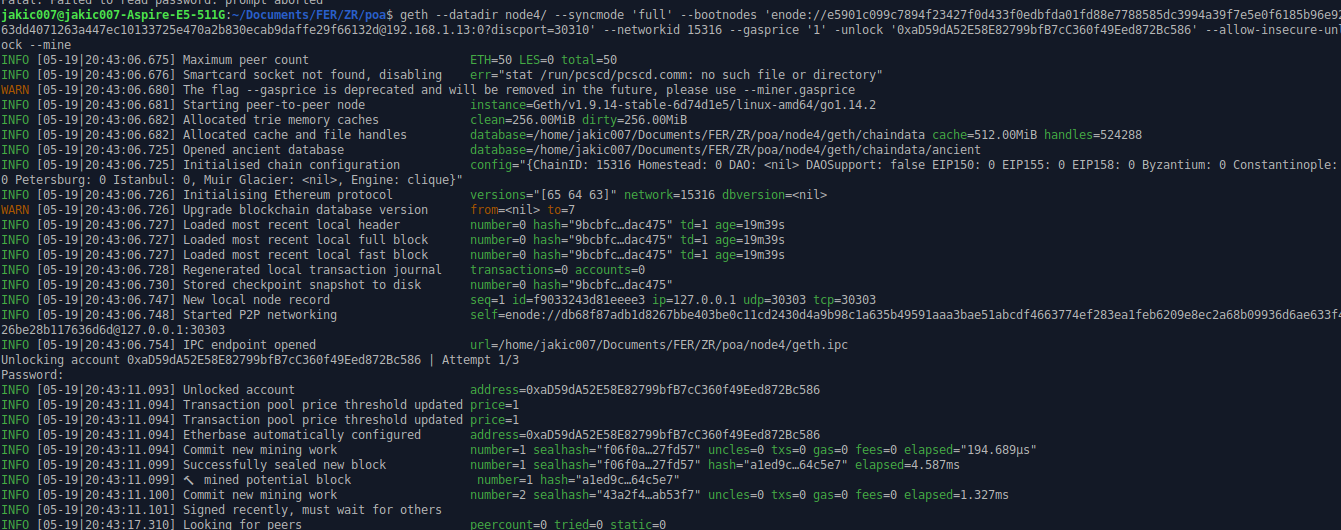
\includegraphics[width=\textwidth]{nodeStart.png}
  \caption{Ispis nakon pokretanja geth procesa}
  \centering
\end{figure}

Iz ispisa se može vidjeti kako je nakon upisane lozinke za otključavanje novčanika pokrenuto rudarenje, odnosno kreiranje blokova.
Kao što je već objašnjeno detaljnije u prethodnom poglavlju, potrebno je imati (N/2)+1 čvorova \emph{online} kako bi se blokovi
kontinuirano stvarali gdje je N broj adresa navedenih u \emph{genesis.json} datoteci. U slučaju da neki čvor \emph{ispadne},
blokovi će se stvarati dokle god je dovoljno aktivnih čvorova. Kad se čvor ponovno poveže, on će uskladiti svoje stanje
s ostalima kako bi povijest bila svugdje jedinstvena. \\
Novi blok se generira svako 15 sekundi jer je tako zadano prilikom incijalizacije \emph{genesis.json} datotekom. \\
U isto se vrijeme na \emph{bootnodeu} vide \emph{ping-pong} poruke čvorova što znači da su svi čvorovi uspješno povezani i međusobno
vidljivi.

\begin{figure}[h]
  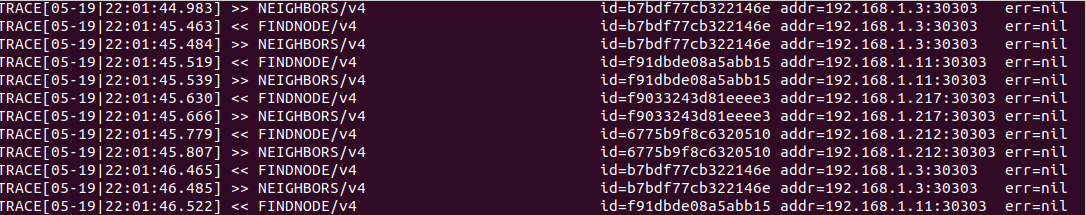
\includegraphics[width=\textwidth]{bootnode.png}
  \caption{Komunikacija čvorova i \emph{bootnodea}}
  \centering
\end{figure}

\pagebreak
\section{Praćenje stanja (engl. \emph{monitoring})}
U prijašnjem odjeljku je pokrenuta potpuno funkcionalna mreža no korisnicima nije jednostavno pratiti stanje gledajući
dnevnike (engl. \emph{logs}) iz komandne linije. Postoji mnogo besplatnih dostupnih i otvorenih alata koji nude jednostavniji
prikaz bitnih podataka u obliku jednostavne web aplikacije koja se povezuje izravno na čvor. Obično se koristi http protokol
ili websocket veza kako bi se podaci dobavljali.
\subsection{Pretražitelj blokova (engl. \emph{block explorer})}
Osnovni dio praćenja stanja je \emph{block explorer}. Pomoću njega se može u realnom vremenu pratiti stanje \emph{blockchaina}
što podrazumijeva prikaz najvišeg trenutnog bloka (engl. \emph{block height}) te pretraživanje i filtriranje transakcija u 
pojedinom bloku. \\
Odabrana je aplikacija \emph{Alethio Ethereum Lite Explorer} zbog svoje jednostavnosti i ažurnosti. To je klijentska
web aplikacija koja se povezuje na bilo koji \emph{Ethereum} čvor koji ima omogućen udaljen poziv procedura (engl. \emph{RPC}). \\
Čvorovi postavljeni u prethodnom dijelu nemaju omogućen udaljen poziv procedura. Da ga omogućili potrebno je zaustaviti geth proces
na odabranom uređaju te ponovno pokrenuti dodavanjem parametara:

\begin{lstlisting}
  --rpc --rpcaddr 'localhost' --rpcport 8545  --rpcapi 'personal,db,eth,net,web3,txpool,miner' --rpccorsdomain "*"
\end{lstlisting}

Ovim postupkom je omogućeno spajanje bilo kojeg servisa s istog računala na naš \emph{geth} proces putem porta 8545 i http protokola.

Postoje dva načina pokretanja ove aplikacije, prevođenjem izvornog koda na vlastitom računalu ili već javno dostupnim
\emph{docker} kontejnerom. Zbog jednostavnosti i niske zahtevnosti, za ovaj projekt je odabran drugi način.
Jedini preduvjet je imati instaliran \emph{docker} klijent na računalu. Nakon toga se sve pokreće jednom naredbom.

\begin{lstlisting}
  $ docker run -p 8080:80 -e APP_NODE_URL="http://localhost:8545" alethio/ethereum-lite-explorer
\end{lstlisting}

\emph{Docker} provjerava postoji li već lokalno dostupna slika te ako ne postoji je dohvaća s \emph{Docker Hub} repozitorija.
Ovim načinom nije potrebno mijenjati konfiguracijsku datoteku već je dovoljno samo dodati varijablu okoline (engl. \emph{environment variable})
koja aplikaciji daje IP adresu i vrata čvora na koji se potrebno spojiti. \\
Parametrom "-p 8080:80" se prosljeđuje \emph{port} 80 unutar kontejnera na \emph{port} 8080 na uređaju na kojem se pokreće kontejner. \\
Utipkavanjem adrese "localhost:8080" u željeni preglednik otvara se aplikacija i prikazuje početni ekran. \\
Blok 47 na slici je prazan, odnosno niti jedna transakcija se nije dogodila u njemu.

\begin{figure}[h]
  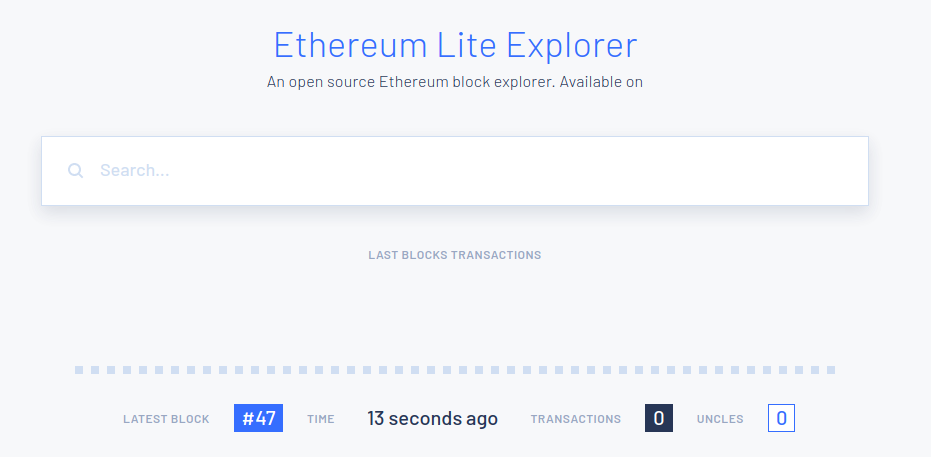
\includegraphics[width=\textwidth]{blockexplorer.png}
  \caption{Početni ekran pretražitelja blokova}
  \centering
\end{figure}

\subsection{Opterećenost čvorova}
Za dobivanje podataka potrebnih za usporedbu performanci na raznorodnom sklopovlju potreban je poseban servis koji će pratiti
opterećenost sklopovlja čvora. Jednako kao i za praćenje stanja blokova, postoji više dostupnih alata. Za ovaj rad je ponovno
odabran \emph{Alethiov} alat \emph{ethstats}. Razlog tome je što je jedini redovno održavan, besplatan i moguće ga je pokrenuti
uz vrlo malo konfiguracije pomoću \emph{docker-composea}. \\
Dovoljno je preuzeti datoteku s poveznice
 \footnote{\url{https://raw.githubusercontent.com/Alethio/ethstats-network-server/master/docker/lite-mode/redis-persistence/docker-compose.yml}} koju 
 treba izmijeniti za ovu konfiguraciju. \\
\emph{Ethstats} se sastoji od više servisa koji čine cjelinu. \emph{Docker-compose} nam olakšava pokretanje te nakon podešavanja
varijabli okruženja unutar \emph{docker-compose.yaml} datoteke moguće je pokrenuti sve servise jednom naredbom.
\begin{lstlisting}
  $ docker-compose up -d
\end{lstlisting}
Time smo pokrenuli \emph{ethstats server}, \emph{dashboard}, \emph{redis} i \emph{deepstream}.
Server pribavlja podatke sa čvorova i sprema ih u \emph{Redis} bazu podataka i istovremeno pruža \emph{dashboardu} i \emph{deepstreamu} koji
su zaduženi za grafički prikaz i analitiku. \\
Pokretanjem prethodne naredbe dobiva se pogreška koja kaže da se server ne može povezati na \emph{ethstats-cli}. \emph{ethstats-cli} 
je odvojeni servis koji se treba pokrenuti na svakom čvoru koji se želi pratiti. On je zaslužan za prikupljanje podataka o iskorištenosti
memorije, procesora i ostalih detalja o sklopovlju. Njegov zatjev je prethodno instaliran \emph{node} verzije novije od 8.11 što se može 
provjeriti naredbom:
\begin{lstlisting}
  $ node -v
\end{lstlisting}
Kad je osigurana odgovarajuća verzija \emph{nodea} moguće je globalno instalirati \emph{ethstats-cli} i pokrenuti naredbama:
\begin{lstlisting}
  $ npm install -g ethstats-cli
  $ ethstats-cli --server-url http://192.168.1.217:3000 -r --account-email jakov.buratovic@fer.hr --node-name pc
\end{lstlisting}
Prvim pokretanjem obavlja se registracija čvora pa je zbog toga unesena adresa e-pošte i proizvoljan naziv čvora. IP adresa u argumentu
"--server-url" jest IP adresa računala na kojem će biti pokrenut \emph{ethstats-server}. U ovom primjeru je to prijenosno računalo. \\
Sada možemo izmijeniti \emph{docker-compose.yaml} datoteku željenim uređivačem teksta. Dovoljno je promijeniti konfiguraciju servisa
\emph{server} na sljedeći način:
\begin{lstlisting}
  server:
    container_name: ethstats-network-server
    image: alethio/ethstats-network-server:latest
    restart: always
    depends_on:
      - deepstream
      - redis
    ports:
      - 127.0.0.1:3000:3000
      - 192.168.1.217:3000:3000
      - 127.0.0.1:3030:3030
      - 127.0.0.1:8888:8888
    environment:
      - NETWORK_ID=15316
      - NETWORK_NAME=dev
\end{lstlisting}

U odnosu na zadanu konfiguraciju, dodano je preusmjeravanje unutarnjeg porta 3000 na vanjsko sučelje računala kako bi ostali uređaji
u lokalnoj mreži mogli vidjeti \emph{ethstats-server} te je izmijenjen identifikator mreže koji je bio postavljen na vrijednost "1" što
označava glavnu Ethereum mrežu \emph{Ethereum mainnet}. Ako ponovno pokrenemo \emph{docker-compose} trebali bismo uspješno biti povezani
na čvorove i posjetom adrese "localhost:80" biti će prikazano sučelje.

\begin{figure}[h]
  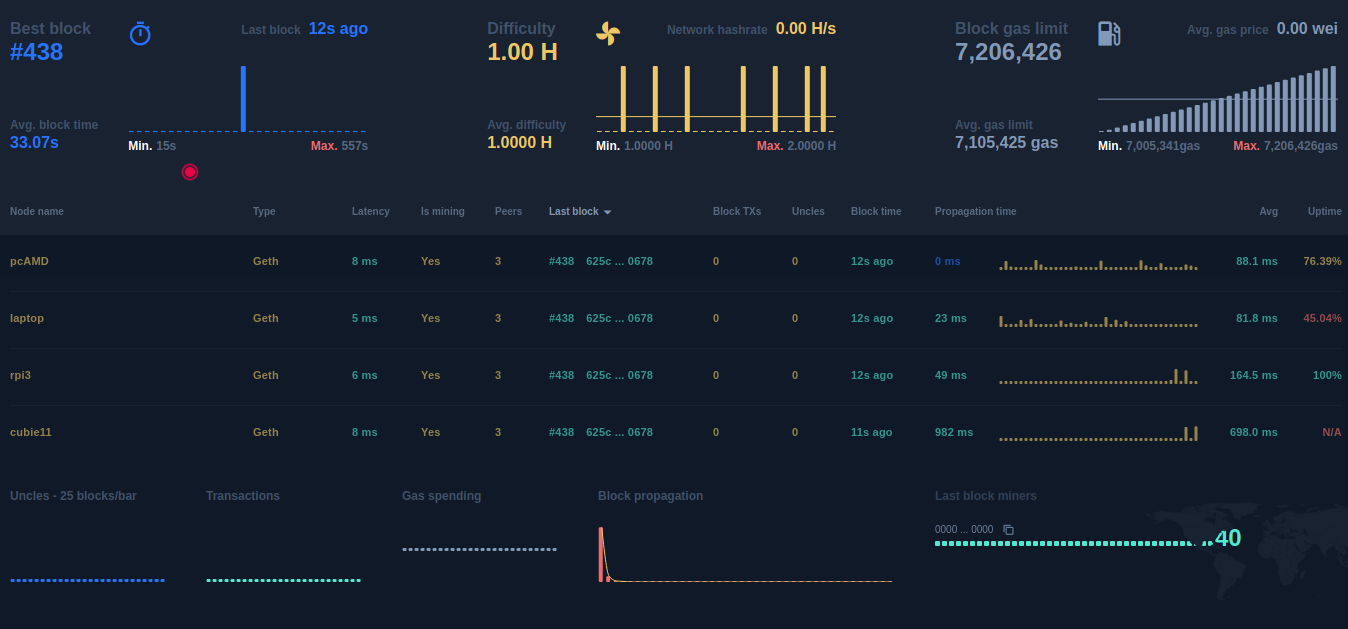
\includegraphics[width=\textwidth]{ethstatsDashboard.png}
  \caption{Sučelje \emph{ethstatsa}}
  \centering
\end{figure}

Kao i u \emph{block exploreru} vidljiv je posljednji blok no ovoga puta uz više detalja i podacima za svaki čvor posebno.
Desno od posljednjeg bloka vidimo statistiku o vremenu kreiranju novih blokova. Minimalno vrijeme je 15 sekundi što odgovara konfiguraciji
no maksimalno vrijeme je 557 sekundi što znači da 557 sekundi nije bilo dovoljno povezanih čvorova u mreži i proizvodnja blokova je stala. \\
Ispod vidimo listu svih čvorova s osnovnim podacima kao što su brzina odaziva, broj povezanih čvorova na taj čvor, posljednji blok na pojedinom
čvoru te brzinu propagiranja novog bloka na čvoru. \\
Iz ove liste vidimo da su svi čvorovi sinkronizirani na istom posljednjem bloku što nam govori da je njihovo sklopovlje dovoljno sposobno
pokretati ovakav tip mreže. Veće opterećenje se može postići skraćivanjem vremena kreiranja blokova i izvršavanjem složenih programskih
kodova pametnih ugovora. \\
Za više detalja potrebno je odabrati čvor čime se otvara novi prikaz u kojem vidimo zauzeće procesora i radne memorije u odabranom
vremenskom razdoblju.
\pagebreak

\begin{figure}[h]
  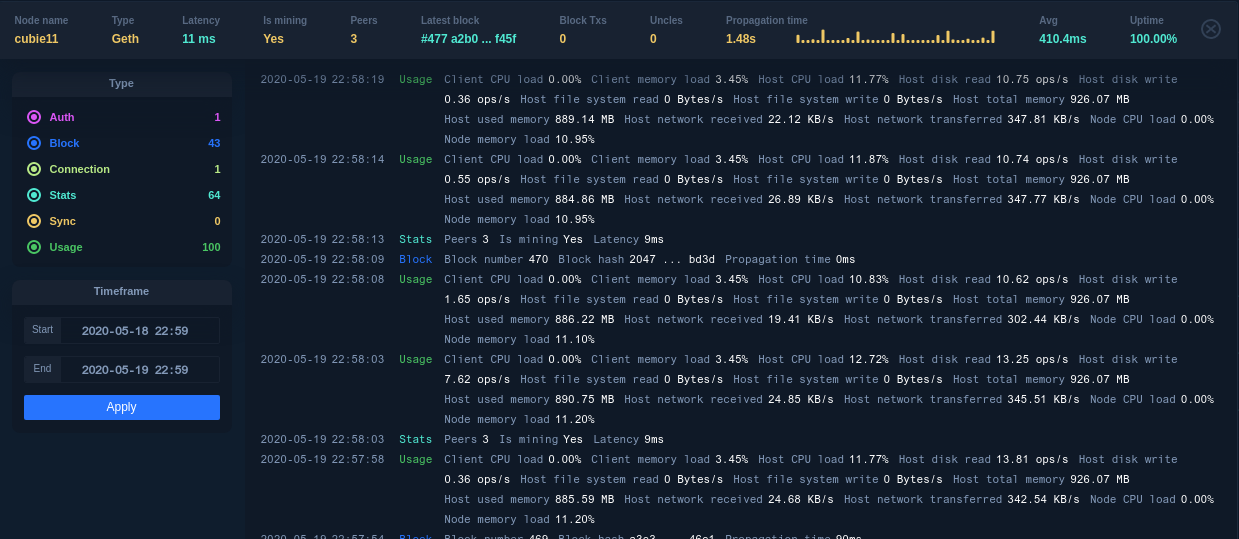
\includegraphics[width=\textwidth]{ethstatsCubie.png}
  \caption{Opterećenost Cubieboard2 pločice}
  \centering
\end{figure}

\emph{Ethstats} je odlično rješenje za nadgledanje više sustava na jednom računalu preko jedinstvenog sučelja. Ako želimo najpreciznije 
moguće podatke u stvarnom vremenu onda je potrebno na pojedinom uređaju pokrenuti neki servis za nadgledanje iskorištenosti resursa kao
na primjer \emph{htop} koji je predinstaliran u većini distribucija \emph{Linuxa} i pokreće se izravno iz terminala. Na grafu niže
je zabilježena prosječna opterećenost procesora na pojedinom uređaju procesom \emph{geth}. Kao što je vidljivo za moderno stolno ili prijenosno računalo opterećenost
je gotovo zanemariva dok se na \emph{single-board} računalima proces pokazao nešto zahtjevniji. Raspberry Pi 1 jedini na ovom grafu ne bi trebalo izravno uspoređivati
jer njegov \emph{geth} proces nije obavljao jednak zadatak kao i na ostalim čvorovima. On nije uopće sinkronizirao blokove niti sudjelovao u njihovom stvaranju nego
je samo služio kao središnja jedinica za pronalaženje čvorova u mreži. Obzirom na njegovo sporije sklopovlje, čak i s tim zadatkom je bio najviše opterećen.

\begin{figure}[h]
  \caption{Iskorištenost procesora}
  \centering
  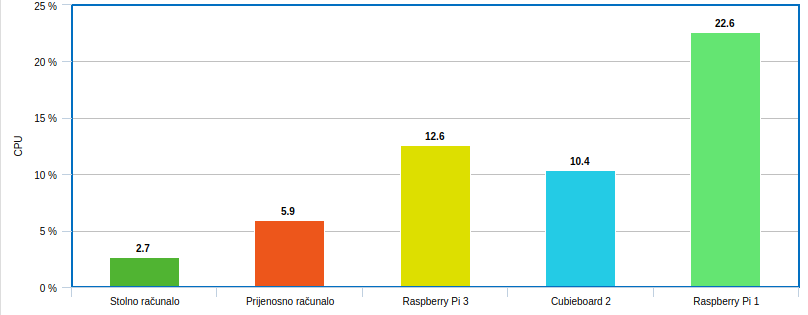
\includegraphics[width=\textwidth]{cpuUtil.png}
\end{figure}

\emph{Htop} nam pruža precizne podatke i o postotku zauzeža radne memorije pojedinim procesom. Ovdje je jasno vidljivo kako je Raspberry Pi 1 imao manje zahtjevan
zadatak te unatoč njegovih 192 MB dostupne memorije, samo je otprilike 20 MB zauzeto \emph{geth} procesom dok na uređajima koji moraju pratiti stanje na \emph{blockchainu}
proces zahtjeva više memorije. Ponovno, za modernija računala ti zahtjevi nisu visoki dok bi na \emph{single-board} računalima memorija mogla predstavljati usko grlo
u nekom složenijem sustavu s više pokrenutih procesa u isto vrijeme.

\begin{figure}[h]
  \caption{Iskorištenost memorije}
  \centering
  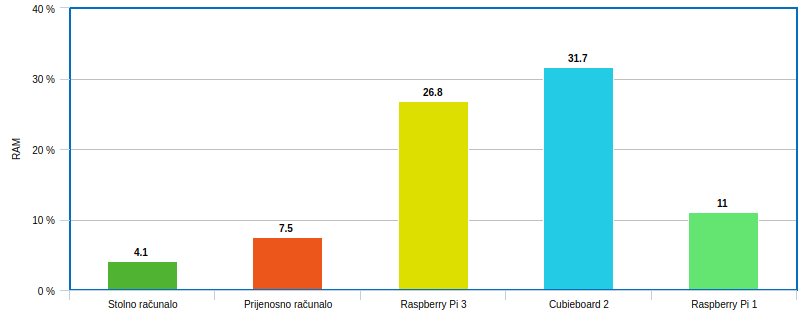
\includegraphics[width=\textwidth]{ramUtil.png}
\end{figure}

\section{Transakcije i pametni ugovori}
Sama mreža nije pretjerano korisna dok su blokovi prazni, odnosno dok se ne odvijaju nikakve transakcije među članovima mreže. Transakcije mogu biti vrlo jednostavne
kao na primjer slanje određene količine \emph{Ethera} s jednog novčanika na drugi ili složenije kao postavljanje programskog koda u obliku pametnog ugovora ili interakcija
s već postavljenim pametnim ugovorom te izvršavanje njegovog koda. \\
Korisnik ima više različitih dostupnih načina izvršavanja transakcija. Najprimitivniji način i isto tako rijetko korišten od strane korisnika jest interakcija putem
naredbenog retka koristeći \emph{geth cli}. Taj način zahtjeva dobro znanje o naredbama i razumijevanje njihovih akcija. \\
Osim naredbenog retka, postoje brojne aplikacije koje se mogu povezati na mrežu putem biblioteke te na način prilagođen njenim zahtjevima nuditi određene mogućnosti
interakcije. Najčešće su te aplikacije pisane u \emph{Javascriptu} i koriste \emph{web3.js}\footnote{\url{https://web3js.readthedocs.io/en/v1.2.8/#}} biblioteku zbog
jednostavne integracije s web aplikacijama za preglednike i vrlo dobre dokumentacije.
Za ovaj rad je odabran \emph{Metamask}\footnote{\url{https://metamask.io/}}, klijentska aplikacija za upravljanje novčanicima i izvođenje i potpisivanje transakcija. 
Dostupna je kao ekstenzija za \emph{Chromium} i \emph{Firefox} preglednike ili kao mobilna \emph{iOS} ili \emph{Android} aplikacija. \\
\subsection{Slanje i primanje Ethera}
Nakon instalacije \emph{Metamask} aplikacije u preglednik, otvara se njeno sučelje te traži korisnika da izradi novi novčanik ili se prijavi s već postojećim.
Kako su prethodno već generirani novčanici koje koriste čvorovi, potrebno je njih ubaciti. Da bismo ubacili postojeći novčanik u metamask potrebno je znati ili
privatni ključ novčanika ili koristiti \emph{json} datoteku koja je automatski izrađena prilikom generiranja novčanika \emph{gethom}. Tajna datoteka se nalazi
u pod direktoriju \emph{keystore}.

\begin{figure}[h]
  \centering
  \begin{minipage}[b]{0.4\textwidth}
    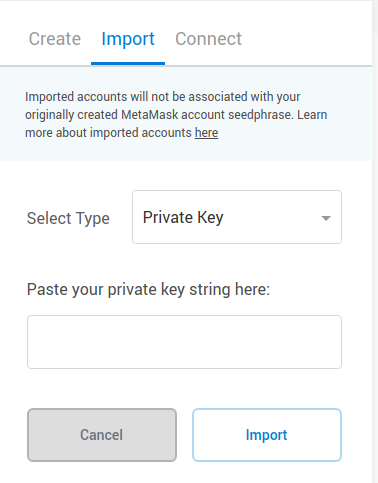
\includegraphics[width=\textwidth]{mmimportprivate.png}
    \caption{Prijava privatnim ključem}
  \end{minipage}
  \hfill
  \begin{minipage}[b]{0.4\textwidth}
    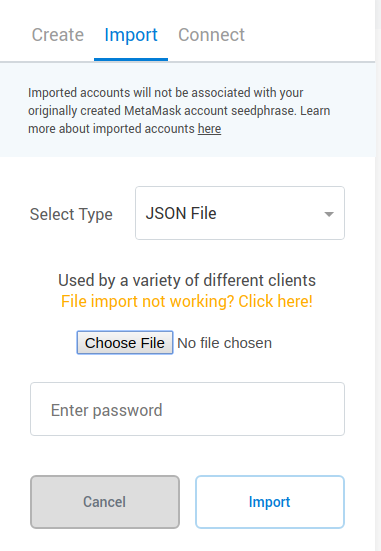
\includegraphics[width=\textwidth]{mmiportjason.png}
    \caption{Prijava datotekom}
  \end{minipage}
\end{figure}

Nakon što je \emph{Metamask} uspješno postavljen novčanikom može se vidjeti da je trenutno stanje 0 ETH. Razlog tome je što je \emph{Metamask} inicijalno povezan
na glavnu \emph{Ethereum} mrežu, \emph{mainnet}. Potrebno je podesiti aplikaciju da bude povezana na neki od čvorova privatne mreže. Treba odabrati \emph{Localhost 8545}
jer je čvor na računalu s \emph{Metamask} klijentom dostupan preko unaprijed zadanog porta 8545. 

\pagebreak

\begin{figure}[h]
  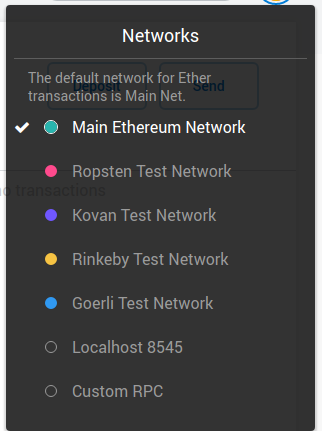
\includegraphics[scale=0.5]{mmnetworkdd.png}
  \caption{Odabir mreže}
  \centering
\end{figure}

Ako se \emph{Metamask} uspješno povezao na čvor, pisat će stanje na novčaniku. To stanje odgovara inicijalnom stanju zadanom u \emph{genesis.json} datoteci ukoliko
nisu već provedene transakcije. Kako je u ovom primjeru zadana vrlo visoka vrijednost koja u primjerice glavnoj mreži ne bi uopće bila moguća, prikaz nije idealno
formatiran no to neće umanjiti funkcionalnosti.

\begin{figure}[h]
  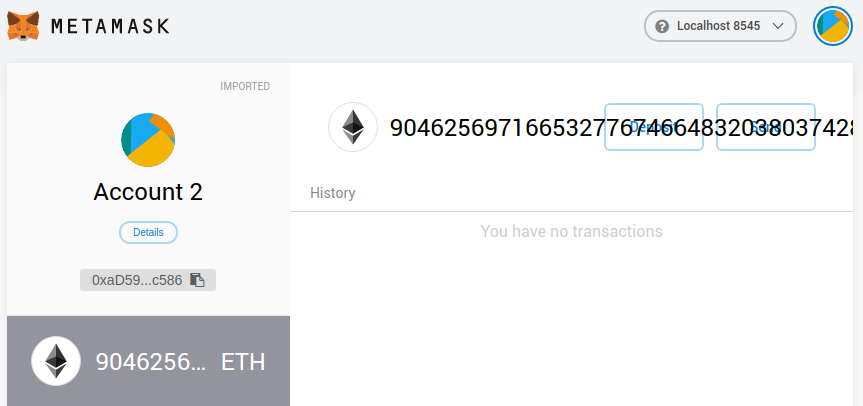
\includegraphics[width=\textwidth]{mmimported.png}
  \caption{Stanje}
  \centering
\end{figure}

Odabirom gumba \emph{Send} otvara se novi prikaz u koji je moguće upisati adresu novčanika primatelja i željeni iznos za transakciju. Ispod polja za upis iznosa
postoji mogućnost odabira provizije koja će biti utrošena prilikom provedbe transakcije. U \emph{proof of authority} ta opcija nije važna, odnosno nema razlike u brzini
izvođenja transakcije. Najbolje je odabrati najnižu vrijednost ili upisati ručno. Te vrijednosti su zanemarive u odnosu na stanje koje je na novčaniku tako da niti veća
provizija neće biti značajna u ovom slučaju. Provizija se dijeli čvorovima u mreži koji su navedeni u \emph{genesis.json} datoteci te tako ostaje u cirkulaciji.

\begin{figure}[h]
  \centering
  \begin{minipage}[b]{0.4\textwidth}
    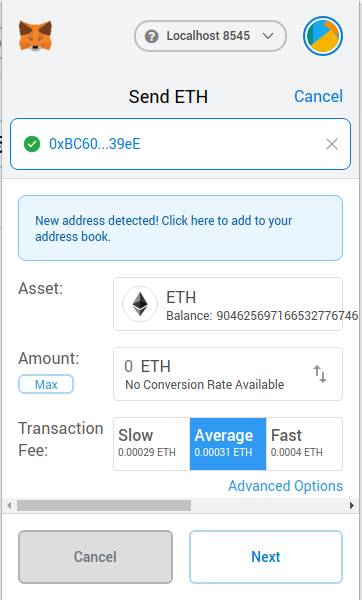
\includegraphics[width=\textwidth]{mmsendtocubie.png}
    \caption{Slanje transakcije}
  \end{minipage}
  \hfill
  \begin{minipage}[b]{0.4\textwidth}
    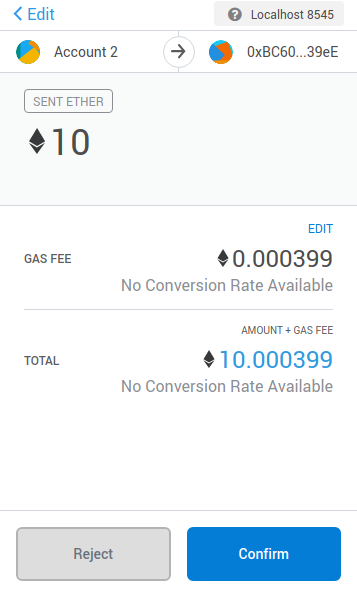
\includegraphics[width=\textwidth]{sent.png}
    \caption{Pregled i potvrda}
  \end{minipage}
\end{figure}

Nakon što je transakcija poslana ona se objavljuje čvoru koji ju provjerava i potom uključuje u idući blok, daje joj identifikator i propagira ju ostalim čvorovima.
U najviše 15 sekundi bi se novi blok trebao stvoriti s tom transakcijom. To će biti jasno vidljivo u pretražitelju blokova. Odabirom bloka i transakcije u njemu se otvara 
prikaz detalja o toj transakciji kao što su identifikator, adrese primatelja i pošiljatelja, iznos koji je poslan i provizija koja je utrošena. U gornjem dijelu postoji
informacija o broju potvrda. To je podatak koji govori koliko je blokova generirano nakon bloka s tom transakcijom.

\pagebreak

\begin{figure}[h]
  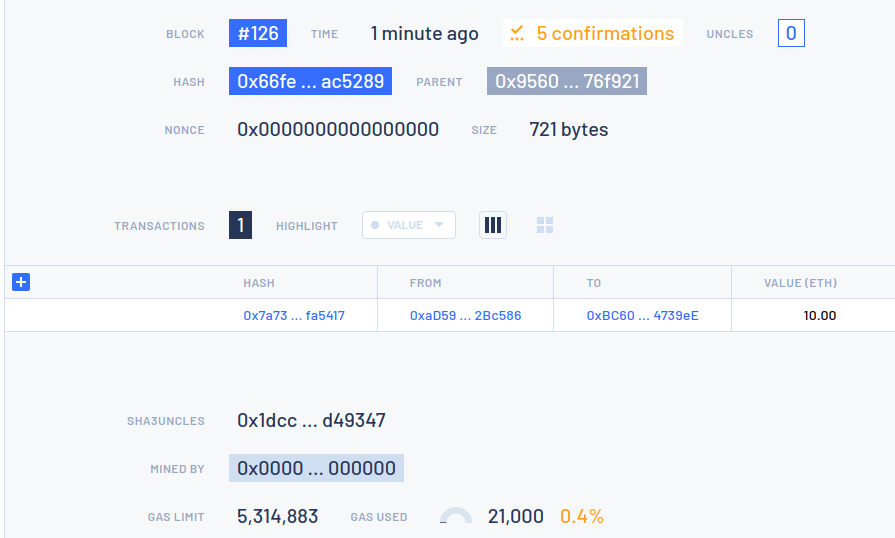
\includegraphics[width=\textwidth]{blocktx.png}
  \caption{Prva transakcija}
  \centering
  \vfill
\end{figure}

\subsection{Pametni ugovori}
Pametni ugovori su ono što Ethereum razlikuje od običnih kriptovaluta koje služe samo za razmjenu vrijednosti putem transakcija. Danas postoji velik broj postavljenih 
pametnih ugovora na glavnoj Ethereum mreži. Postavaljanje pametnog ugovora je transakcija kojom se šalje prevedeni kod pametnog ugovora na \emph{blockchain}.
Kod se piše u objektno orjentiranom jeziku \emph{Solidity} i prevodi koristeći \emph{solc}, prevoditelj za Solidity. Prevođenjem programskog koda dobiva se binarna datoteka
i aplikacijsko binarno sučelje (engl. \emph{ABI - application binary interface}). \emph{ABI} služi kao sučelje za interakciju s pametnim ugovorom. Nakon što je kod
proveden potrebno je postaviti produkte prevođenja na \emph{blockchain}.
\subsubsection{Kod i prevođenje}
Najjednostavniji način za isprobati \emph{Solidity} i pametne ugovore je koristeći službeni \emph{Ethereumov IDE Remix}\footnote{\url{https://remix.ethereum.org/}}. 
To je web aplikacija koja se također može povezati na bilo koji \emph{Ethereum} čvor ali i naravno na glavnu mrežu u kojoj je moguće pisati programski kod
pametnih ugovora u \emph{Solidity} programskom jeziku. Iz iste aplikacije je moguće korištenjem ugrađenih dodataka prevesti taj kod i postaviti ga na mrežu.
Upravo iz tog razloga je idealan alat za brzo isprobavanje ili testiranje pametnih ugovora jer nije potrebno postavljati kompleksna razvojna okruženja. \\
Otvaranjem početne stranice, s lijeve strane je prikazan pretražitelj datoteka. Tu se nalazi nekoliko jednostavnih primjera pametnih ugovora koji su dovoljni
za demonstriranje samog toka događaja pa iz tog razloga za ovaj rad nije pisan nikakav kompleksniji kod. \emph{Solidity} datoteke imaju nastavak \emph{.sol}
pa ih je lako prepoznati. \\
Za ovaj rad će se koristiti prvi primjer \emph{1\_Storage.sol} pa ga je potrebno otvoriti s dva klika kako bi se prikazao njegov izvorni kod.
U prvom liniji koda definirane su valjane verzije \emph{Solidity} jezika u kojima će se ovaj kod možći uspšješno prevesti. To je vrlo važno jer je jezik
nov i vrlo brzo izlaze nova izdanja koja mijenjaju bitne stvari pa iz tog razloga starija sintaksa neće biti valjano prevedena s novijim prevoditeljem. Također je moguće
navesti raspon verzija kao što je u ovom primjeru stavljeno. \\
Nakon definiranja verzije, ključnom riječi \emph{contract} definira se naziv ugovora. Kako je \emph{Solidity} objektno orjentiran jezik, ta ključna riječ odgovara 
riječi \emph{class} u primjerice \emph{Java} jeziku. Unutar tijela ugovora se definiraju metode i varijable. Metode mogu biti označene s ključnom riječi \emph{view} što
znači da ta metoda ne upisuje ništa na \emph{blockchain} nego samo pribavlja i čita podatke s njega. Izvođenje takvih metoda je besplatno za razliku od metoda koje
upisuju podatke. Svako upisivanje na \emph{blockchain} zahtjeva transakciju koja mora biti uključena u blok što košta. \\
Ovaj ugovor ima dvije vrlo jednostavne metode. Jedna metoda upisuje broj na \emph{blockchain}, a druga vraća posljednji upisan broj. 
Varijabla \emph{uint256 number} je varijabla koja je pohranjena u memoriji samog ugovora. Metoda \emph{store} prima kao argument \emph{uint256} broj koji postavlja 
varijablu ugovora na unesenu vrijednost. \\
Nakon što je kod napisan portebno je s lijeve strane odabrati \emph{Solidity compiler} dodatak koji služi za prevođenje koda. U prikazu se odabire verzija prevoditelja
i ugovor koji korisnik želi prevesti. Odabirom gumba \emph{Compile 1\_Storage.sol}, ugovor je uspješno preveden.

\begin{figure}[h]
  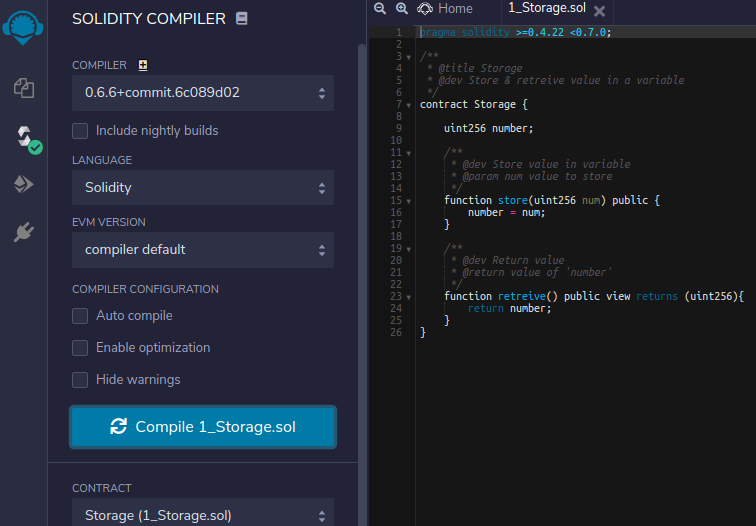
\includegraphics[width=\textwidth]{remixcompiled.png}
  \caption{Prevođenje pametnog ugovora}
  \centering
  \vfill
\end{figure}

\pagebreak

Dobivene produkte prevođenja treba postaviti na \emph{blockchain}. U izborniku s lijeve strane treba odabrati dodatak \emph{Deploy and run transactions} što otvara
prikaz u kojem se odabire okolina. Ukoliko u izborniku nije dostupan taj dodatak potrebno je odabrati posljednju stavku u izborniku, upravitelj dodacima (engl. \emph{Plugin manager})
u čije s polje za pretraživanje može upisati ključna riječ \emph{deploy} i aktivirati dodatak pritiskom na gumb \emph{activate}.
Dostupne su tri okoline, \emph{Javascript VM, Injected Web3} i \emph{Web3} provider. \\
\emph{Javascript VM} je virutalni stroj koji se izvodi u pregledniku i ne spaja se na stvarne čvorove. To je dobra opcija za testiranje ispravnosti koda prije postavljanja
na mrežu. Za potrebe ovog rada može poslužiti bilo koja od preostale dvije opcije. Odabirom \emph{Web3 Provider} opcije, \emph{Remix} se izravno spaja na čvor dok odabir
\emph{Injected Web3} opcije podrazumijeva da korisnik ima postavljen \emph{Metamask} ili neki drugi novčanik u pregledniku koji onda upravlja pozivima i transakcijama.
Ako je odabran \emph{Web3 Provider} onda treba u istom prikazu odabrati \emph{Ethereum} račun koji će se koristiti za postavljanje ugovora i ograničenje potrošnje
\emph{gasa}. U slučaju da se koristi \emph{Metamask}, otvara se novi prozor u kojem se od korisnika traži dozvola korištenja \emph{Metamaska} od strane \emph{Remixa}.
Račun i ograničenje \emph{gasa} se podešavaju u istom prozoru nakon odabira gumba \emph{Deploy} u \emph{Remixu}. \\

\begin{figure}[h]
  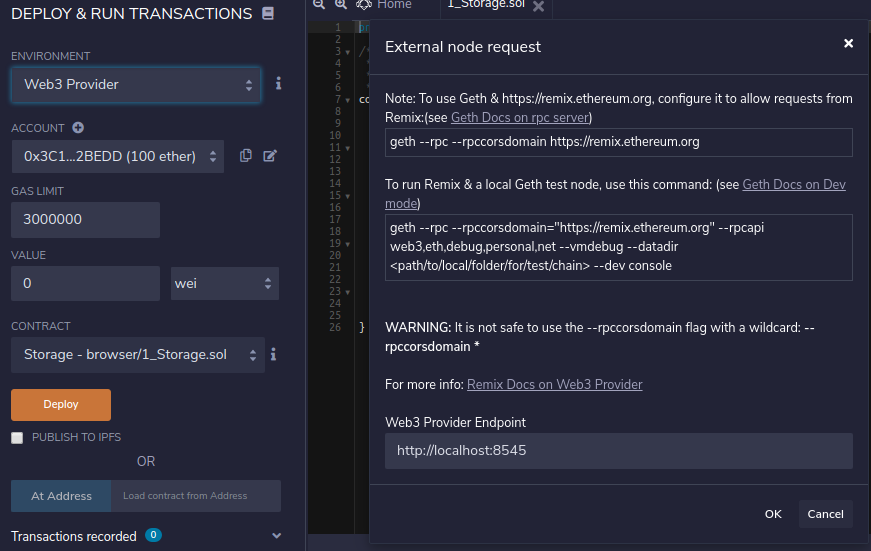
\includegraphics[width=\textwidth]{remixconnect.png}
  \caption{Postavljanje ugovora}
  \centering
  \vfill
\end{figure}

U idućem bloku je uključena transakcija koja kreira ugovor na jedinstvenoj adresi, odnosno ugovor posjeduje svoj novčanik čiji je vlasnik sam ugovor. 
U ovom trenutku je moguće izvršavati programski kod ugovora s bilo kojeg člana mreže jer se on replicirao na svaki čvor prilikom sinkronizacije posljednjeg bloka.
Vrijednosti varijabli i rezultati izvršavanja metoda ugovora su također usklađeni u svakom čvoru što je vrlo korisna funkcionalnost. Nitko ne može mijenjati stanje
bez da to svi ostali znaju. \\
U \emph{Remixu} se pojavljuje novi izbornik koji služi za pozivanje metoda psotavljenog ugovora. Vidi se metoda \emph{store} i \emph{retreive}. Kao što je i napisano
u kodu, prva metoda prima broj tipa \emph{uint256} te ga postavlja u varijablu pametnog ugovora u idućem bloku. Ta se transakcija plaća vrlo malim iznosom \emph{gasa}
jer je to operacija upisivanja na \emph{blockchain}. Operacija \emph{retreive} je operacija čitanja što znači da se ona neće pojaviti kao transakcija i potpuno je 
besplatna. 

\pagebreak

\begin{figure}[h]
  \centering
  \begin{minipage}[b]{0.4\textwidth}
    \includegraphics[width=\textwidth]{remixfunctions.png}
    \caption{Raspoložive metode}
  \end{minipage}
  \hfill
  \begin{minipage}[b]{0.4\textwidth}
    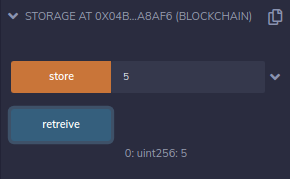
\includegraphics[width=\textwidth]{number5retreived.png}
    \caption{Dohvaćanje vrijednosti}
  \end{minipage}
\end{figure}

\subsubsection{Primjer složenijeg ugovora}

U ovom ugovoru je dozvoljeno bilo kome mijenjati vrijednost varijable. U nekim slučajevima to je željena mogućnost. Za neki drugu funkcionalnost je možda poželjno da
samo određeni računi smiju upisivati, a svi ostali čitati. Dobar primjer malo složenijeg ugovora je lutrija. \\
Jednostavan primjer ugovora za lutriju bi dozvoljavao da bilo tko može igrati, odnosno uložiti \emph{Ether} na adresu pametnog ugovora ali da nitko ne može pokrenuti
izvlačenje sretnog dobitnika osim vlasnika ugovora, odnosno računa koji je postavio ugovor na \emph{blockchain}. Pokretanjem metode za izvlačenje dobitnika nasumično
se bira jedna adresa novčanika iz liste svih koji su sudjelovali u tom krugu lutrije te se njemu isplaćuje cjelokupan sadržaj novčanika ugovora. Nakon toga se lista
novčanika prazni i kreće novi krug lutrije. \\
Ugovor bi bio još bolji kad bi se potpuno izbacio utjecaj vlasnika jer igrači nemaju nikakvu garanciju da će vlasnik ikada pokrenuti izvlačenje. To se može napraviti
tako da se u kodu napiše da se izvlačenje pokreće samostalno primjerice kad je dovoljan broj različitih novčanika igrao ili kad je dostignuto dovoljno stanje na računu
samog ugovora.






\chapter{Zaključak}
Zaključak.

\bibliography{literatura}

\bibliographystyle{fer}

\begin{sazetak}
Sažetak na hrvatskom jeziku.

\kljucnerijeci{Ključne riječi, odvojene zarezima.}
\end{sazetak}

% TODO: Navedite naslov na engleskom jeziku.
\engtitle{Performance Comparison of the Ethereum Blockchain on Heterogeneous Hardware}
\begin{abstract}
Abstract.

\keywords{Keywords.}
\end{abstract}

\end{document}
